\section{Line Track}
Den linjefølgende robot følger en bestemt bane ved at anvende princippet om at modtage et konstant signal. Signalet sendes fra lyssensoren med en varierende værdi afhængig af farven på den kørte overflade. 
\newline
Den forudbestemte bane er defineret ved en sort bane med en minimusbredde på 30 mm omgivet af hvid eller gråtonet omkringliggende farve. 
\newline
Gruppen har valgt som fremgangsmåde først at anvende én sensor til at sende den værdi som læses fra den kørte overflade. 

\begin{figure}[h!]
  \centering
  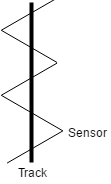
\includegraphics[width=0.2\textwidth]{figures/sensorAlgoritme.png}
  \caption{Sensor algoritme over én sensor}
\end{figure}

På ovenstående figur ses det hvordan sensoren registrerer den omkringliggende farve og drejer til højre. Herfra fortsætter bilen indtil den optegnede bane igen registreres og der igen læses en hvidnuanceret farve efter stregen. Da den hvidtonede overflade registreres på ny justerer bilen retning mod venstre for at kunne følge linjen.  
\newline

\subsection{Videreudvikling af Line Track}
For at gøre bilen i stand til at kunne følge linjen efter bedste og hurtigst mulige evne har gruppen valgt at implementere yderligere sensore. Dette tillader bilen at kunne følge en lige linje samt være i stand til at registrere fremadkomne ændringer i banens forløb.
\newline
På nedenstående figur ses hvordan implemengtering af flere sensorer hjælper bilen i at bestemme banens forløb.

\begin{figure}[h!]
  \centering
  \includegraphics[width=0.8\textwidth]{figures/linjeAlgoritme.png}
  \caption{Sensoralgoritme over tre implementeret sensorer}
  \label{line_track}
\end{figure}

Ved anvendelse af tre sensorer skabes fire mulige scenarier som bilen skal være i stand til at forholde sig til.

\begin{enumerate}
   \item Scenarie
   \begin{itemize}
     \item Her ses det hvordan de tre sensorer tilgår banens forløb. Det antages at bilen følger en lige linje hvor den midterste sensor registrere den sortnuanceret overflade. De to yderste sensorer registrere en anden overflade som er ens på begge sider og bilen skal derfor ikke justere retning.
   \end{itemize}
   \item Scenarie
   \begin{itemize}
     \item Her registrere venstre sensor banens forløb hvilket indikerer at banens forløb har ændret sig. Den midterste og den højre sensor registrere begge den hvidtonede overflade og bilen skal derfor justere ind til venstre for at den midterste sensor igen læser den mørke overflade så bilen igen kører en lige linje. 
     \end{itemize}
        \item Scenarie
   \begin{itemize}
     \item Ligesom 2. scenarie registrerer her én af ydersensorne at banens forløb har ændret sig. Højre sensor registrerer den mørke overflade hvoraf de to andre sensorer registrerer den hvidtonede overflade. Herfra skal bilens retning ligeledes ændres så den miderste sensor læser den mørke overflade igen. 
   \end{itemize}
           \item Scenarie
   \begin{itemize}
     \item I dette scenaie antages at en uforudset hindring eller hændelse har påvirket sensor eller banens forløb. Dette kan eksempelvis være fejlregistrering fra sensor eller snavs eller misfarvninger på den opstillede bane. 
     \newline
     Ingen af sensorerne er i stand til at videresende en registreret måling af den pågældende overflade og bilen kan derved ikke registrere hvor den opstillede bane er. I dette scenarie står bilen derfor stille. 
   \end{itemize}
\end{enumerate}

